\chapter{量子情報理論}

\begin{ex}
    \label{ex12.1}
    $\braket{\psi|\phi} = 0$であれば,
    \begin{align*}
        U\ket{0} = \ket{\psi}, U\ket{1} = \ket{\phi}
    \end{align*}
    なるユニタリ$U$が存在して,
    \begin{align*}
        \Qcircuit @C=1em @R=1em {
        \lstick{}        & \gate{U^\dagger} & \ctrl{1} & \gate{U} & \qw \\
        \lstick{\ket{0}} & \qw              & \targ    & \gate{U} & \qw \\
        }
    \end{align*}
    という回路を用いれば, $\ket{\psi}\ket{\psi}, \ket{\phi}\ket{\phi}$という状態を作り出せる.
\end{ex}

\begin{ex}
    \label{ex12.2}
    \begin{align*}
        \tr \left[
            \sum_y
            \left(\sqrt{E_y} \otimes U_y \right)\left( \sigma \otimes \ket{0}\bra{0} \right)\left(\sqrt{E_y} \otimes U_y^\dagger\right)
            \right]
         & =
        \tr \left[
            \sum_y
            \left(\sqrt{E_y} \sigma \sqrt{E_y} \right) \otimes \ket{y}\bra{y}
            \right]
        \\
         & =
        \sum_y\tr \left[\sqrt{E_y} \sigma \sqrt{E_y} \otimes \ket{y}\bra{y}
            \right]
        \\
         & =
        \sum_y\tr \left[\sigma E_y\right] =
        \tr \sigma = \tr \left[
            \sigma \otimes \ket{0}\bra{0}
            \right].
    \end{align*}
\end{ex}

\begin{ex}
    \label{ex12.3}

\end{ex}

\begin{ex}
    \label{ex12.4}
\end{ex}

\begin{ex}
    \label{ex12.5}
    定理12.2(1)より, ある$\epsilon$を固定して,
    \begin{align*}
        \forall \delta > 0 \ \exists n_0 \in \mathbb{N} \ \forall n \ge n_0 \ \ P\left( X \in T(n, \epsilon) \right) \ge 1 - \delta
    \end{align*}
    である. 1情報記号のデータ圧縮に必要なビット数$A(n, \epsilon)$として,
    \begin{align*}
        A(n,\epsilon) & =
        H(X) P \left(X \in T(n,\epsilon) \right) + \frac{\log d^n}{n} P \left(X \notin T(n,\epsilon) \right)
        \\
                      & \le
        R  P \left(X \in T(n,\epsilon) \right) + \log d \left(1 - P \left(X \in T(n,\epsilon) \right)\right)
        \\
                      & \le
        R + \delta \log d
    \end{align*}
    なので,
    \begin{align*}
        \forall \delta > 0 \ \exists n_0 \in \mathbb{N} \ \forall n \ge n_0 \ \ |A(n,\epsilon)-R| \le \delta \log d.
    \end{align*}
\end{ex}

\begin{ex}
    \label{ex12.6}
    \begin{align*}
        C_X = p^{4 - \wt{X}} (1-p)^{\wt{X}}
    \end{align*}
\end{ex}

\begin{ex}
    \label{ex12.7}
    コラム12.4で, $V=I$とすれば良い.
\end{ex}

\begin{ex}
    \label{ex12.8}
    定理12.6の証明の式(12.51)で式(9.141)を用いて,
    \begin{align*}
        \bar{F} \ge F\left( \rho^{\otimes n}, D^n \circ C^n\right)
    \end{align*}
    すれば良い.
\end{ex}

\begin{ex}
    \label{ex12.9}
    (1)\
    $X$の確率分布関数を
    \begin{align*}
        p_X(0) = q, \ p_X(1) = 1 - q
    \end{align*}
    とすると$Y$の確率分布関数は
    \begin{align*}
        p_Y(0) = q(1-p), \ p_Y(1) = (1-q)(1-p),\  p_Y(e) = p
    \end{align*}
    となるので,
    \begin{align*}
        H(X:Y)
         & = H(Y) - H(Y|X)                                                                        \\
         & = H(Y) - \sum_x p_X(x) H(Y|X=x)                                                        \\
         & = H(Y) - H_{bin}(p)                                                                    \\
         & = -q(1-p)\log q(1-p) - (1-q)(1-p)\log(1-p)(1-q) - p \log p + p \log p + (1-p)\log(1-p) \\
         & =(1-p) H_{bin}(q) \le (1-p) H_{bin}(1/2) = 1 - p
    \end{align*}
    を得るので, 消去チャンネルの容量は$1-p$.
    \par
    (2)\
    \begin{align*}
        p = H_{bin}(p)
    \end{align*}
    を満たす非ゼロの$p$を$p_0$とする. $p\le p_0$であれば, $p \le H_{bin}(p)$なので, $1 - H_{bin}(p) \le 1 - p$.
    \begin{figure}[H]
        \begin{center}
            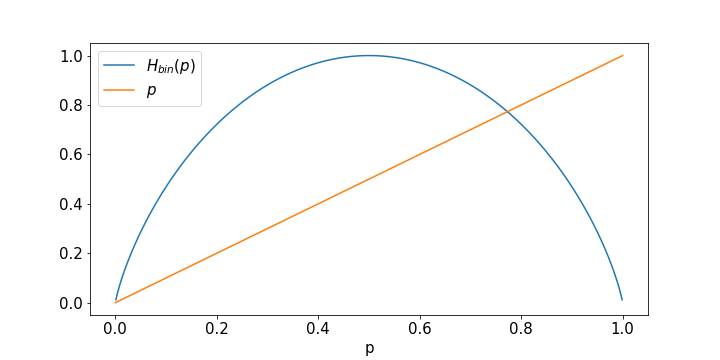
\includegraphics[width = 80mm]{./fig/ex12_9.png}
        \end{center}
    \end{figure}
\end{ex}

\begin{ex}
    \label{ex12.10}
    \begin{align*}
        X \xrightarrow{\mathscr{N}_1} Y \xrightarrow{\mathscr{N}_2} Z
    \end{align*}
    として,
    \begin{align*}
        C \left( \mathscr{N}_1 \circ \mathscr{N}_2 \right) = \max_{p_X(x)} H(X:Z) \\
        C \left( \mathscr{N}_1 \right) = \max_{p_X(x)} H(X:Y)                     \\
        C \left( \mathscr{N}_2 \right) = \max_{p_Y(y)} H(Y:Z)
    \end{align*}
    であることと, 定理11.5より,
    \begin{align*}
        C \left( \mathscr{N}_1 \circ \mathscr{N}_2 \right)
        \le \min \left(C \left( \mathscr{N}_1 \right), C \left( \mathscr{N}_2 \right)\right)
    \end{align*}
    を得る.
\end{ex}

\begin{ex}
    \label{ex12.11}
    \begin{align*}
        \chi \left( \qo \right) = \max_\rho \max_{\left\{ p_j,
            \rho_j \right\} \mathrm{ \ subject \ to} \ \rho = \sum_j p_j \rho_j }
        \left[ S\left( \qo(\rho)\right) - \sum_j p_j S\left( \qo(\rho_j) \right) \right]
    \end{align*}
    とかけることに注目する.
    \par
    まず, $\rho$を固定する.
    \begin{align*}
        \rho_j = \sum_k q_j^k \ket{\psi_j^k}\bra{\psi_j^k}
    \end{align*}
    とすると, エントロピーの凹性と$\qo$の線型性より,
    \begin{align*}
        S \left( \qo(\rho_j)\right) \ge
        \sum_k q_j^k S \left( \qo(\ket{\psi_j^k}\bra{\psi_j^k}) \right)
    \end{align*}
    を得る. 式(11.79)より, この等号成立条件が$\rho_j$が純粋状態の時であることから,
    \begin{align*}
        \max_{\left\{ p_j,
            \rho_j \right\} \mathrm{ \ subject \ to} \ \rho = \sum_j p_j \rho_j }
        \left[ S\left( \qo(\rho)\right) - \sum_j p_j S\left( \qo(\rho_j) \right) \right]
    \end{align*}
    を実現するアンサンブル$\{p_j, \rho_j \}$は純粋状態だけからなることがわかる.
    \par
    次に, $\rho = \sum_j p_j \rho_j$を動かす. 任意の$\rho$は, 独立な純粋状態$\rho_1,\ \rho_2 , ..., \rho_{d^2}$の線形和でかけることから, $\max$を取るべきアンサンブルとしては, 高々$d^2$個の純粋状態だけからなるアンサンブルを考えれば十分.
\end{ex}

\begin{ex}
    \label{ex12.12}
\end{ex}

\begin{ex}
    \label{ex12.13}
    $\qo$が$\qo_1, \qo_2$を用いて,
    \begin{align*}
        \qo = p \qo_1 + ( 1 - p) \qo_2
    \end{align*}
    とかけるとする. 入力$\rho$に対する$\qo, \qo_1, \qo_2$のw行列を$W, W_1, W_2$とすると,
    \begin{align*}
        W = p W_1 + (1-p) W_2
    \end{align*}
    を得る.よって, エントロピーの凹性より,
    \begin{align*}
        S \left( \rho, p \qo_1 + (1-p)\qo_2 \right)
        =
        S(pW_1 + (1-p)W_2 )
        \ge
        p S(W_1) + (1-p) S(W_2)
        =
        p S \left( \rho, \qo_1\right) + (1-p) S \left( \rho, \qo_2\right).
    \end{align*}
\end{ex}

\begin{ex}
    \label{ex12.14}
    $Q$は量子コンピュータのqubit全体, $Q_1$は$Q$のうち誤り訂正可能な符号とし, $Q_2 = Q - Q_1$と書く. この時, 定理12.10の証明で議論したように, 
    \begin{align*}
        Q_1 が誤り訂正可能 
        &\longleftrightarrow
        \rho^{R Q_2} = \rho^{R} \otimes \rho^{Q_2}  \ (\because 定理12.10の証明での議論)\\
        &\longleftrightarrow
        S\left( \rho^{Q_1 Q_2}\right)
        =
        S\left( \rho^R\right)
        =
        S\left( \rho^{Q_2}\right) -  S\left( \rho^{RQ_2}\right) = S\left( \rho^{Q_2}\right) -  S\left( \rho^{Q_1}\right)\\
        &\longleftrightarrow
        \rho^{Q_1 R} = \rho^{Q_1} \otimes \rho^R \ \ (\because 式(11.78)の等号成立)
    \end{align*}
\end{ex}

\begin{ex}
    \label{ex12.15}
    1つの例として, 強い劣加法性
    \begin{align*}
        S\left( \rho^{R'' E_1'' E_2''}\right) + S\left( \rho^{E_1''}\right)
        \le S\left( \rho^{R'' E_1''}\right) + S\left( \rho^{E_1'' E_2''}\right)
    \end{align*}
    から関係式を導いてみる.
    上の強い劣加法性から, 定理12.10の第2不等号が導かれたことを思い出すと,
    \begin{align*}
        S\left(\rho''\right) - S\left(\rho'\right)
        \le
        S\left( \rho, \qo_2 \circ \qo_1\right)
        -
        S\left( \rho, \qo_1\right)
        =
        S\left( \rho^{E_1'' E_2''} \right) - S\left( \rho^{E_1''}\right).
    \end{align*}
    ここで, $\rho^{E_1'' E_2''}$,$\rho^{E_1''}$を$\qo_1, \qo_2$の演算要素$\{ E_i \}, \{ F_i\}$で書くことを考える. 量子演算を作用させる前の$QE_1'' E_2''$の状態$\rho^Q \otimes \ket{0}\bra{0} \otimes \ket{0}\bra{0}$とすると,
    \begin{align*}
        \rho^{Q E_1'' E_2''}
        =
        \sum_{i,j,k,l}  F_i E_j \rho^Q E_k^\dagger F_l^\dagger \otimes \ket{j} \bra{k} \otimes \ket{i}\bra{l}
    \end{align*}
    なので,
    \begin{align*}
        \rho^{E_1'' E_2''}
         & = \tr_Q \rho^{Q E_1'' E_2''}
        = \sum_{i,j,k,l}  \tr_Q \left[ F_i E_j \rho^Q E_k^\dagger F_l^\dagger \right] \ket{j} \bra{k} \otimes \ket{i}\bra{l}
        \\
        \rho^{E_1'' }
         & = \tr_{Q E_2} \rho^{Q E_1'' E_2''}
        =\sum_{i,j,k}  \tr_Q \left[ F_i E_j \rho^Q E_k^\dagger F_i^\dagger \right] \ket{j} \bra{k}
    \end{align*}
    \par
    他の組み合わせについては, arXiv:quant-ph/0011036に示してある.
    \par
\end{ex}

\begin{ex}
    \label{ex12.16}
    定理12.10の第1等号の成立条件で示した.
\end{ex}

\begin{ex}
    \label{ex12.17}
    示すべきは,
    \begin{align*}
        \forall t \in \mathbb{R} \ \
        \sum_{j=1}^d \max\left( x_j - t, 0\right)
        \le
        \sum_{j=1}^d \max\left( y_j - t, 0\right)
        \longleftrightarrow
        \forall k \in \{1, 2, ..., d \} \ \
        \sum_{j=1}^k x_j^\downarrow
        \le
        \sum_{j=1}^k y_j^\downarrow
    \end{align*}
    \par
    $\longrightarrow)$
    $k = 1,2, ..., d$ に対して$t = y_k^\downarrow$とすれば,
    \begin{align*}
        \sum_{j=1}^k \left( y_j^\downarrow -  y_k^\downarrow\right)
        =
        \sum_{j=1}^d \max\left( y_j^\downarrow  -  y_k^\downarrow, 0\right)
        \ge
        \sum_{j=1}^d \max\left( x_j^\downarrow -  y_k^\downarrow, 0\right)
        \ge
        \sum_{j=1}^k \max\left( x_j^\downarrow -  y_k^\downarrow, 0\right)
        \ge
        \sum_{j=1}^k \left(x_j^\downarrow  - y_k^\downarrow \right)
    \end{align*}
    より
    \begin{align*}
        \sum_{j=1}^k y_j^\downarrow
        \ge
        \sum_{j=1}^k x_j^\downarrow
    \end{align*}
    を得る.
    \par
    $\longleftarrow)$
    任意の実数$t$をとってくると,
    \begin{enumerate}
        \item $\exists i \in \{ 1,2, ..., d-1\} \ \  x_i^\downarrow \ge t \ge x_{i+1}^\downarrow$
        \item $t \ge x^\downarrow_1$
        \item $x^\downarrow_d \ge t$
    \end{enumerate}
    のいずれかを満たし, いずれの場合でも
    \begin{enumerate}
        \item $ \sum_{j=1}^d \max(x_j - t, 0)
                  =
                  \sum_{j=1}^i (x_j^\downarrow - t)
                  \le
                  \sum_{j=1}^i (y_j^\downarrow - t)
                  \le
                  \sum_{j=1}^i \max(y_j^\downarrow - t,0)
                  \le
                  \sum_{j=1}^d \max(y_j - t,0)$
        \item $\sum_{j=1}^d \max(x_j - t, 0) = 0 \le \sum_{j=1}^d \max(y_j - t,0)$
        \item $ \sum_{j=1}^d \max(x_j - t, 0)
                  =
                  \sum_{j=1}^d (x_j^\downarrow - t)
                  \le
                  \sum_{j=1}^d (y_j^\downarrow - t)
                  \le
                  \sum_{j=1}^d \max(y_j - t,0)$
    \end{enumerate}
    のように,
    \begin{align*}
        \sum_{j=1}^d \max\left( x_j - t, 0\right)
        \le
        \sum_{j=1}^d \max\left( y_j - t, 0\right)
    \end{align*}
    が示せた.
\end{ex}

\begin{ex}
    \label{ex12.18}
    $x^1 , x^2 \prec y$, $ 0 \le \lambda \le 1$とすると,
    $k = 1, 2, ..., d$に対して,
    \begin{align*}
        \sum_{j=1}^k \lambda x_j^{1 \downarrow} + (1-\lambda) x_j^{2 \downarrow}
        \le
        \sum_{j=1}^k y_j^\downarrow
    \end{align*}
    であり,
    \begin{align*}
        \sum_{j=1}^d \lambda x_j^{1 \downarrow} + (1-\lambda) x_j^{2 \downarrow}\le
        \sum_{j=1}^d y_j^\downarrow
    \end{align*}
    であるので, $\lambda x_j^{1} + (1-\lambda) x_j^{2} \prec y$なので, $\{x | x \prec y\}$は凸集合.
\end{ex}

\begin{ex}
    \label{ex12.19}
    示すべきは, $x \prec y$ならば$x' \prec y'$, つまり$l = 1,2, ..., d-1$に対して,
    \begin{align*}
        \sum_{i=1}^l x_i'^\downarrow
        \le
        \sum_{i=1}^l y_i'^\downarrow
    \end{align*}
    が成立し, $l = d-1$で等号が成立すること.
    \par
    次のような$k$を定める;
    \begin{align*}
        y_1^\downarrow \le y_2^\downarrow \le ... \le y_k^\downarrow \le (1-t) y_1^\downarrow + t y_j^\downarrow \le y_{k+1}^\downarrow \le y_{k+2}^\downarrow \le ... \le y_{j}^\downarrow
        \le ... \le y_d^\downarrow
    \end{align*}
    また, $l = 1,2, ..., d-1$として,
    \begin{align*}
        \sum_{i=1}^l x_i'^\downarrow
        =
        \sum_{i=1}^{l+1} x_i^\downarrow - x_1^\downarrow
        \le
        \sum_{i=1}^{l+1} y_i^\downarrow - t y_1^\downarrow - (1-t)y_j^\downarrow
    \end{align*}
    が成立.
    \par
    \underline{$l \le k -1 $のとき}\
    \begin{align*}
        \sum_{i=1}^l y_i'^\downarrow = \sum_{i=2}^{l+1} y_i^\downarrow
    \end{align*}
    なので,
    \begin{align*}
        \sum_{i=1}^l x_i'^\downarrow
        \le
        \sum_{i=1}^{l+1} y_i^\downarrow - t y_1^\downarrow - (1-t)y_j^\downarrow
        =
        \sum_{i=1}^l y_i'^\downarrow + (1-t)y_1^\downarrow - (1-t)y_j^\downarrow
        \le
        \sum_{i=1}^l y_i'^\downarrow +  y_{k+1}^\downarrow - y_j^\downarrow
        \le
        \sum_{i=1}^l y_i'^\downarrow.
    \end{align*}
    \par
    \underline{$k \le l \le j - 1 $のとき}\
    \begin{align*}
        \sum_{i=1}^l y_i'^\downarrow = \sum_{i=2}^{l} y_i^\downarrow + (1-t) y_1^\downarrow + t y_j^\downarrow
    \end{align*}
    なので,
    \begin{align*}
        \sum_{i=1}^l x_i'^\downarrow
        \le
        \sum_{i=1}^{l+1} y_i^\downarrow - t y_1^\downarrow - (1-t)y_j^\downarrow
        =
        \sum_{i=1}^l y_i'^\downarrow - y_j^\downarrow + y_{l+1}^\downarrow
        \le
        \sum_{i=1}^l y_i'^\downarrow
    \end{align*}
    \par
    \underline{$j \le l $のとき}\
    \begin{align*}
        \sum_{i=1}^l y_i'^\downarrow = \sum_{i=2}^{j-1} y_i^\downarrow + \sum_{i=j+1}^{l+1} y_i^\downarrow + (1-t) y_1^\downarrow + t y_j^\downarrow
        =
        \sum_{i=2}^{l+1} y_i^\downarrow + (1-t) y_1^\downarrow - (1- t)  y_j^\downarrow
    \end{align*}
    なので,
    \begin{align*}
        \sum_{i=1}^l x_i'^\downarrow
        \le
        \sum_{i=1}^{l+1} y_i^\downarrow - t y_1^\downarrow - (1-t)y_j^\downarrow
        =
        \sum_{i=1}^l y_i'^\downarrow
    \end{align*}
    \par
    \underline{$l = d - 1 $のとき}\
    \begin{align*}
        \sum_{i=1}^{d-1} x_i'^\downarrow
        =
        \sum_{i=1}^{d} y_i^\downarrow - t y_1^\downarrow - (1-t)y_j^\downarrow
        =
        \sum_{i=1}^l y_i'^\downarrow
    \end{align*}
\end{ex}

\begin{ex}
    \label{ex12.20}
    $\rho_\psi$の台をAliceの状態空間とすれば良い.
\end{ex}

\begin{ex}
    \label{ex12.21}
    \begin{align*}
        \tr_B \ket{\psi}\bra{\psi}
         & = 0.4 \ket{0}\bra{0} + 0.4 \ket{1}\bra{1} + 0.1 \ket{2}\bra{2} + 0.1 \ket{3}\bra{3}
        \\
        \tr_B \ket{\phi}\bra{\phi}
         & = 0.5 \ket{0}\bra{0} + 0.25 \ket{1}\bra{1} + 0.25 \ket{2}\bra{2}
    \end{align*}
    より, $\tr_B \ket{\psi}\bra{\psi} \nprec \tr_B \ket{\phi}\bra{\phi}$
    なので, 定理12.25より$\ket{\psi}$から$\ket{\phi}$への変換はLOCCではできない.
\end{ex}

\begin{ex}
    \label{ex12.22}

\end{ex}

\begin{ex}
    \label{ex12.23}
    教科書の議論より, LOCCにより, $\ket{\psi} = \sum_x \sqrt{x} \ket{x_A}\ket{x_B}$から$S(\rho_\psi)$個のBell状態が作れることがわかっている. ここで, $\rho_\psi = \tr_A \ket{\psi}\bra{\psi}$.
    LOCCによって$S (< S(\rho_\psi))$のBell状態から$\ket{\psi}$が作れるとすると, $S(\rho_\psi)$個のBell状態が作れる. つまり, LOCCによって, $S (< S(\rho_\psi))$のBell状態から $S(\rho_\psi)$個のBell状態が作れる事になるが, これは演習\ref{ex12.24}より矛盾. したがって, 教科書にあるもつれの希釈手続きが最適である.
\end{ex}

\begin{ex}
    \label{ex12.24}
    純粋状態$\ket{\psi}, \ket{\phi}$は,
    \begin{align*}
        \ket{\psi} = \sum_{i=1}^{\mathrm{Sch}(\lambda_\psi)} \sqrt{\lambda_{\psi i}}\ket{i}_A \ket{i}_B , \
        \ket{\phi} = \sum_{i=1}^{\mathrm{Sch}(\lambda_\phi)} \sqrt{\lambda_{\phi i}}\ket{\tilde{i}}_A \ket{\tilde{i}}_B
    \end{align*}
    とかける. ここで,
    \begin{align*}
        \sum_{i=1}^{\mathrm{Sch}(\lambda_\psi)} \lambda_{\psi i}^\downarrow
        = \sum_{i=1}^{\mathrm{Sch}(\lambda_\phi)} \lambda_{\phi i}^\downarrow= 1                     \\
        \forall i \in \{ 1,2, ..., \mathrm{Sch}(\lambda_\psi) \} \ \ \lambda_{\psi i}^\downarrow > 0 \\
        \forall i \in \{ 1,2, ..., \mathrm{Sch}(\lambda_\phi) \} \ \ \lambda_{\phi i}^\downarrow > 0
    \end{align*}
    である.
    定理12.25より, LOCCにより$\ket{\psi} \to \ket{\phi}$という変換が可能であるとすると, $\lambda_\psi \prec \lambda_\phi$. もし, $\mathrm{Sch}(\lambda_\psi) < \mathrm{Sch}({\lambda_\phi})$とすると,
    \begin{align*}
        0 =
        \sum_{i=1}^{\mathrm{Sch}(\lambda_{\psi})} \lambda_{\psi i}^\downarrow
        -
        \sum_{i=1}^{\mathrm{Sch}(\lambda_{\phi})} \lambda_{\phi i}^\downarrow
        =
        \sum_{i=1}^{\mathrm{Sch}(\lambda_{\psi})} ( \lambda_{\psi i}^\downarrow - \lambda_{\phi i}^\downarrow)
        +
        \sum_{i=\mathrm{Sch}(\lambda_{\psi})+1}^{\mathrm{Sch}(\lambda_{\phi})} \lambda_{\phi i}
        > 0
    \end{align*}
    と矛盾. したがって, LOCCによる$\ket{\psi} \to \ket{\phi}$という変換によって, Schmidt数は増加しない.
    \par
    $d$次元状態空間上の純粋状態$\ket{\psi}, \ket{\phi}$が,
    \begin{align*}
        \ket{\psi} & = \left( \frac{\ket{00} + \ket{11}}{\sqrt{2}}\right)^{\otimes k} \ket{\mathrm{ABがもつれてない2qubit状態}}^{\otimes{d-k}}  \\
        \ket{\phi} & =  \left( \frac{\ket{00} + \ket{11}}{\sqrt{2}}\right)^{\otimes l} \ket{\mathrm{ABがもつれてない2qubit状態}}^{\otimes{d-l}}
    \end{align*}
    とする. $\ket{\psi}, \ket{\phi}$はそれぞれAliceとBobが$k, l$個のBell状態を共有している. ここで, $k < l$とすると, $\mathrm{Sch}(\lambda_\psi) = 2^k < \mathrm{Sch}(\lambda_\phi) = 2^l$なので, $\ket{\psi} \to\ket{\phi}$という変換はLOCCによってできない. つまり, AliceとBobの共有するBell状態の数は,LOCCで増加しない.
\end{ex}

\begin{ex}
    \label{ex12.25}
    秘密鍵$n!/2$, 公開鍵$2n$.
\end{ex}

\begin{ex}
    \label{ex12.26}
    $(b_k,b_k') = (0,0)$のとき, Bobは$\ket{\psi_{{a_k}0}} = \ket{a_k}$を$Z$の固有状態を基底とした測定を行い, 測定値$a_k'$は確率1で$a_k$と等しくなる. $(b_k,b_k') = (1,0)$のとき, Bobは$\ket{\psi_{{a_k}1}} = \ket{a_k}$を$Z$の固有状態を基底とした測定を行い, 測定値$a_k'$は確率1/2で$a_k$, 確率1/2で$\bar{a}_k$というようにランダムに得られる. $(b_k,b_k') = (0,1),(b_k,b_k') = (1,1)$のときも同様.
\end{ex}

\begin{ex}
    \label{ex12.27}
    (1) \
    \begin{align*}
        \epsilon = \mu - 2 \delta \ge 0
    \end{align*}
    とする. 2nビットのうち$\mu n$ビットが誤ってるとする. $2n$ビットから$n$ビットの検査ビットを選んだ時に, 検査ビット中の誤りが$\delta n$より小さくなる確率$p$は,
    \begin{align*}
        p = \sum_{i=0}^{\delta n - 1} \frac{{}_{\mu n} C _{i} \times {}_{2n - \mu n} C _{n - i}}{{}_{2n} C_n}.
    \end{align*}
    ここで,
    \begin{align*}
        a_i \equiv {}_{\mu n} C _{i} \times {}_{2n - \mu n} C _{n - i}
    \end{align*}
    とすると, $i = 0, 1, ..., \delta n - 2$に対して,
    \begin{align*}
        \frac{a_{i+1}}{a_i} = \frac{
            \frac{n+1}{i+1} - 1
        }{
            \frac{n+1}{\mu n - i } - 1
        }
        > 1
    \end{align*}
    より, $a_i$は単調増加なので,
    \begin{align*}
        p =
        \sum_{i=0}^{\delta n - 1} \frac{a_i}{{}_{2n} C_n} <
        \delta n \frac{a_{\delta n}}{{}_{2n} C_n} <
        \delta n
        \frac{{}_{\mu n} C _{\delta n} \times {}_{2n - \mu n} C _{n - \delta n}}{{}_{2n} C_n}
    \end{align*}
    を得る.
    \par
    (2)\
    \begin{align*}
        \frac{b}{a} = t, an = s
    \end{align*}
    とすると,
    \begin{align*}
        2^{an H \left( \frac{b}{a}\right)} & = \left[ t^{t} (1-t)^{1-t}\right]^{-s} \\
        {}_{an} C_{bn}                     & = {}_s C_{st}
    \end{align*}
    とかける.
    スターリングの公式より,
    \begin{align*}
        \frac{\sqrt{2 \pi}}{e^2} \frac{s^{s + \frac{1}{2}}}{(st)^{st + \frac{1}{2}} (s(1-t))^{s(1-t) + \frac{1}{2}}}
        \le
        \frac{s!}{(st)! (s - st)!}={}_s C_{st}
        \le
        \frac{e}{2 \pi} \frac{s^{s + \frac{1}{2}}}{(st)^{st + \frac{1}{2}} (s(1-t))^{s(1-t)+ \frac{1}{2}}}.
    \end{align*}
    よって,
    \begin{align*}
        \frac{2^{an H \left( \frac{b}{a}\right)}}{{}_{an} C_{bn}}
         & =
        \frac{\left[ t^{t} (1-t)^{(1-t)}\right]^{-s}}{{}_s C_{st}}
        \\
         & \ge
        \frac{2 \pi}{e}
        \frac{(st)^{st + \frac{1}{2}} (s(1-t))^{s(1-t)+ \frac{1}{2}}}{s^{s + \frac{1}{2}} \left[ t^{t} (1-t)^{1-t}\right]^s}
        \\
         & =
        \frac{2 \pi}{e}
        \left(
        \frac{st \cdot s(1-t)}{s}
        \right)^{\frac{1}{2}}
        \left(
        \frac{(st)^t (s(1-t))^{1-t}}{s t^t (1-t)^{1-t}}
        \right)^{s}
        =
        \frac{2 \pi}{e}
        \sqrt{st(1-t)}
    \end{align*}
    よって, 任意の$t$に対して,
    \begin{align*}
        s > \frac{e^2}{4 \pi^2 t(1-t)}
    \end{align*}
    を満たす程十分大きな$s$を取れば,
    \begin{align*}
        \frac{2^{an H \left( \frac{b}{a}\right)}}{{}_{an} C_{bn}} \ge 1.
    \end{align*}
    もう一方の不等号についても同様に示せる.
    \par
    (3)\
    問題文で与えられた不等式と(2)で示した不等式より,
    \begin{align*}
        p
         & <
        \delta n
        \frac{{}_{\mu n} C _{\delta n} \times {}_{2n - \mu n} C _{n - \delta n}}{{}_{2n} C_n}
        \\
         & <
        \delta n (2n+1) \frac{
            2^{\mu n \left( 1 - 2 \left(  \frac{\mu}{\delta} - \frac{1}{2}\right)^2\right)}
            2^{(2 - \mu )n \left( 1 - 2 \left(  \frac{2 - \mu}{ 1 - \delta} - \frac{1}{2}\right)^2\right)}
        }
        {
            2^{\frac{n}{2}}
        }
        \\
         & =
        \delta n (2n+1) 2^{\frac{3n}{2}}
        2^{-2 n \left( \mu \left(\frac{\mu}{\delta} - \frac{1}{2}\right)^2
                + (2 - \mu) \left(\frac{2 - \mu}{ 1 - \delta} - \frac{1}{2}\right)^2 \right)}
        \\
         & =
        \delta n (2n+1) 2^{\frac{3n}{2}}
        2^{
                -\frac{n}{2}
                \left[
                    \mu \frac{\epsilon^2}{\delta^2}
                    +  (2 - \mu)\frac{(2\epsilon + 3 (1 - \delta))^2}{ (1 - \delta)^2}
                    \right]
            }
        \\
         & <
        \delta n (2n+1) 2^{\frac{3n}{2}}
        2^{
                -\frac{n}{2}
                \left[
                    \mu \frac{\epsilon^2}{\delta^2}
                    +  (2 - \mu)\frac{4 \epsilon^2}{ (1 - \delta)^2}
                    \right]
            }
        \\
         & <
        \delta n (2n+1) 2^{\frac{3n}{2}}
        2^{
                -\frac{n}{2}
                \left[
                    \mu {\epsilon^2}
                    +  (2 - \mu){4 \epsilon^2}
                    \right]
            }
        \\
         & <
        \delta n (2n+1)
        2^{
                -\frac{n}{2}
                \left[
                    3 + (8 - 3 \mu) \epsilon^2
                    \right]
            }
        = 2^{- O (\epsilon^2 n)}.
    \end{align*}
\end{ex}

\begin{ex}
    \label{ex12.28}
    $(a', b) = (0, 1)$のとき, Bobが状態$\ket{\psi}$を$Z$基底で測定して, 固有値$+1$の方を得る. このとき$\ket{\psi} = \ket{0}$つまり$a = a' = 0$. \ $(a', b) = (1, 1)$のときも同様に示せる
\end{ex}

\begin{ex}
    \label{ex12.29}
\end{ex}

\begin{ex}
    \label{ex12.30}
    $\ln(1-x)$のTaylor展開
    \begin{align*}
        \ln(1-x) = -x + O(x^2)
    \end{align*}
    を用いて, 
    \begin{align*}
        S(\rho_\mathrm{max})
        &=
        -(1-2^{-s}) \log(1 - 2^{-s}) - 2^{-s} \log \frac{2^{-s-2n}}{1 - 2^{-2n}}
        \\
        &=
        \frac{1 - 2^{-s}}{\ln 2} \left( 2^{-s} + O(2^{-2s})\right)
        +
        2^{-s}\left( s + 2n\right) + 2^{-s}\left( - 2^{-n} + O(2^{-2n})\right)
        \\
        &=
         \left(2n + s + \frac{1}{\ln2} \right)2^{-s} + O(2^{-2s}).
    \end{align*}
    最後の等号では$s<n$を用いた.
\end{ex}

\begin{ex}
    \label{ex12.31}
    Eveがチャンネル全ての制御ができるとすると, AliceがBobに送信した情報を, 
    \begin{align*}
        F\left( \rho, \ket{\beta_{00}}^{\otimes n} \right) > 1 - 2^{-s}
    \end{align*}
    を満たすように
    \begin{align*}
        \rho = \sum_x p_x \rho_x
    \end{align*}
    と書き換えることができてしまう. $\rho$をAliceとBobがPOVM$\{ E_y\}$によって測定して得た結果$Y$とEveが持っている$\rho$に関する情報$X$の相互情報量は, Holevo限界, エントロピーの非負性, 演習\ref{ex12.30}より, 
    \begin{align*}
        H(X:Y) \le S(\rho) - \sum_x p_x S \left(\rho_x \right) \le S(\rho) 
        < \left(2n + s + \frac{1}{\ln2} \right)2^{-s} + O(2^{-2s}).
    \end{align*}
\end{ex}

\begin{ex}
    \label{ex12.32}
    例えば, ビット反転については, 
    \begin{align*}
        \Pi_{bf} = \frac{I \otimes I - Z \otimes Z}{2}, I - \Pi_{bf} = \frac{I \otimes I + Z \otimes Z}{2}
    \end{align*}
    とかけるので.
\end{ex}

\begin{ex}
    \label{ex12.33}
\end{ex}

\begin{ex}
    \label{ex12.34}
\end{ex}

\begin{ex}
    \label{ex12.35}
\end{ex}

\begin{ex}
    \label{ex12.36}
    明らか.
\end{ex}